\subsection{Functions - relations between sets}
    \subsubsection{Sets}
        Modern algebra starts from the notion of a set. A set $S$ is a collection of elements:
        \begin{equation}
            S = \set{s_1, s_2, \dots, s_n} \thinspace .
        \end{equation}
        Some examples of sets are the set of natural numbers $\N$, the set of real numbers $\R$, the set of complex numbers $\C$. We can also have smaller sets, for example
        \begin{equation}
            S = \set{0, 1} \thinspace ,
        \end{equation}
        being the set of the numbers $0$ and $1$. Sets don't necessarily have to contain only numbers. We can, for example, collect all invertible $n \times n$-matrices in a set:
        \begin{equation}
            \GLg(n, \mathbb{R}) = \set{A \in \mathbb{R}^{n \times n} ; \text{$A$ is invertible}} \thinspace ,
        \end{equation}
        in which the symbol $\GLg$ has to do with `general linear', but more on that when we encounter the general linear group. \\

        The previous examples are all concrete (i.e. not abstract) examples of sets. Now say we have a mathematical object, called $E$ (we haven't specified anything about it), we can say that
        \begin{equation}
            G = \set{E}
        \end{equation}
        is also a set, but in a more abstract sense than the previous examples. We can enlarge this set by adding the elements $C_2, \sigma_v$ and $\sigma_v'$, to end up with
        \begin{equation}
            G = \set{E, C_2, \sigma_v, \sigma_v'} \thinspace ,
        \end{equation}
        in which we still haven't specified anything about the nature of its elements, but in mathematics that is perfectly fine. \\

    \subsubsection{Functions - introduction}
        Naturally, if we have two different sets, we would like to be able to define relations between their elements. This is exactly what a function does. A function (or map, mapping, these are all synonyms) is a relation between two sets $X$ and $Y$:
        \begin{equation} \label{eq:def_function}
            f: X \rightarrow Y: x \mapsto y = f(x) ,
        \end{equation}
        subject to the important condition that every input $x \in X$ is related to exactly one output $y \in Y$. We would read the definition in equation (\ref{eq:def_function}) as follows: $f$ is a function from the set $X$ to the set $Y$, in which every $x \in X$ is related to a $y \in Y$, which we call $f(x)$. \\

        We give special names to the sets $X$ and $Y$, depending on which role they play in the function. The set $X$ is called the domain of the function: it is the set of all inputs for the function. The set $Y$ is then called the function's codomain: it is the set of values that \emph{could} occur as output values for the function. We can then define another set, $Z$, which is called the image of the function: it is the set of \emph{actual} values for the outputs. A visual clarification of the terms can be found in Figure \ref{fig:functions}. \\
        \begin{figure}[H] \centering
            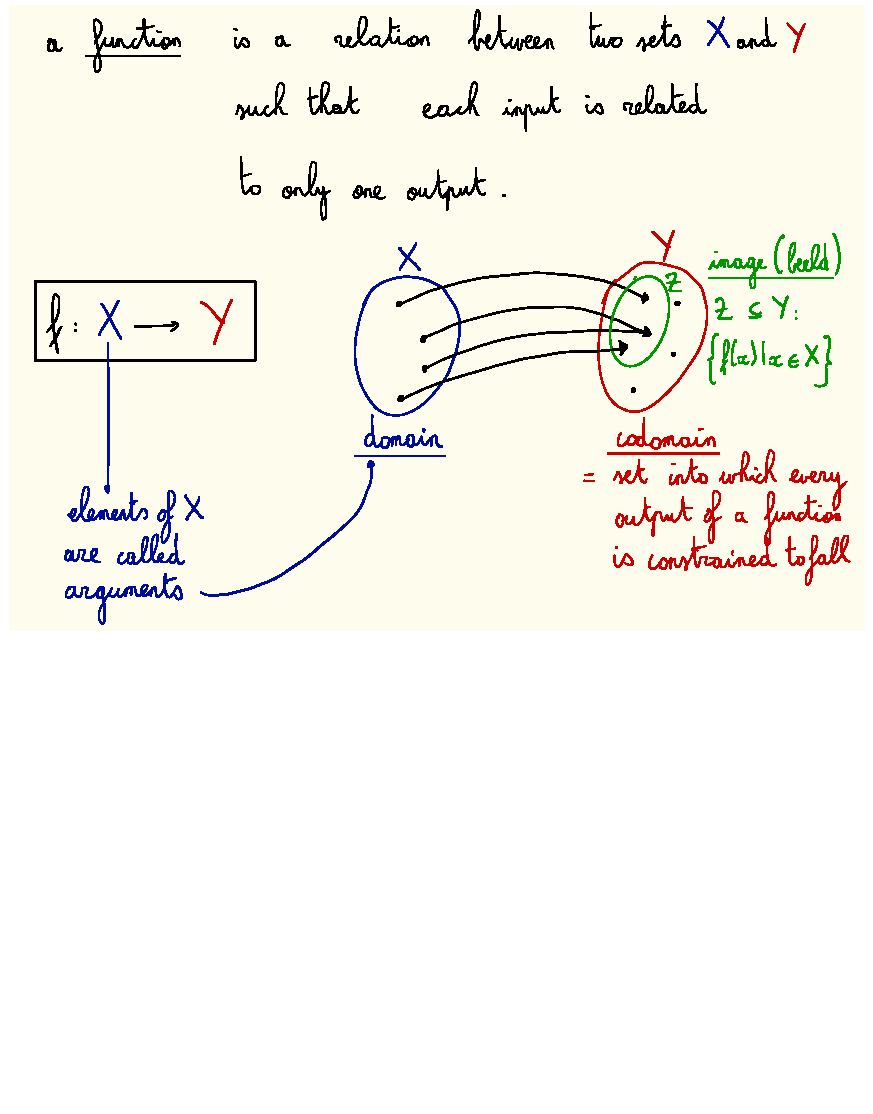
\includegraphics{images/functions}
            \caption{The definition of a function, and a visual clarification of the terms domain, codomain and image. The domain is the set of input values, the codomain is the set of possible output values, and the images is the set of actual output values.}
            \label{fig:functions}
        \end{figure}

        An example of a function could be:
        \begin{equation}
            f: \R \rightarrow \R: x \mapsto f(x) = x^2 + 2
        \end{equation}
        Its domain is $\R$, and its codomain is also $\R$. Here, we can also see the difference between the codomain and the image. The codomain of this function is defined to be $\R$, but its image $[2, +\infty[$. Another example is shown in Figure \ref{fig:function_color}.
        \begin{figure}[H] \centering
            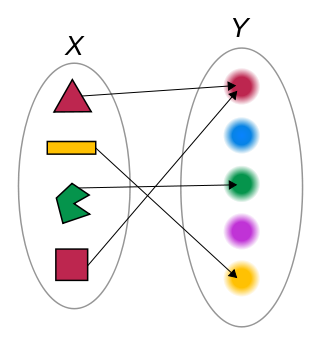
\includegraphics[scale=0.4]{images/function_color}
            \caption{An example of a function that maps an object to its color.}
            \label{fig:function_color}
        \end{figure}
        The reason why this is a function is because every input element of the set $X$, being shapes in a certain color, is related to its color, represented as elements of the set $Y$. In this case, $Y$, the codomain is the set of colors depicted as elements of $Y$, and the range is the set of colors red, green and yellow. \\

        We have seen some examples of functions already, but what are some examples of non-functions? There are actually two requirements to the definition of a function:
        \begin{enumerate}
            \item Every input (element of the domain) has to be related to an output (element of the codomain)
            \item No two outputs (elements of the codomain) may be related to the same input (element of the domain)
        \end{enumerate}
        With these two criteria in mind, it is possible to come up with many examples of relations between two sets that are not functions, for example those shown in Figure \ref{fig:non_functions}.
        \begin{figure}[H] \centering
            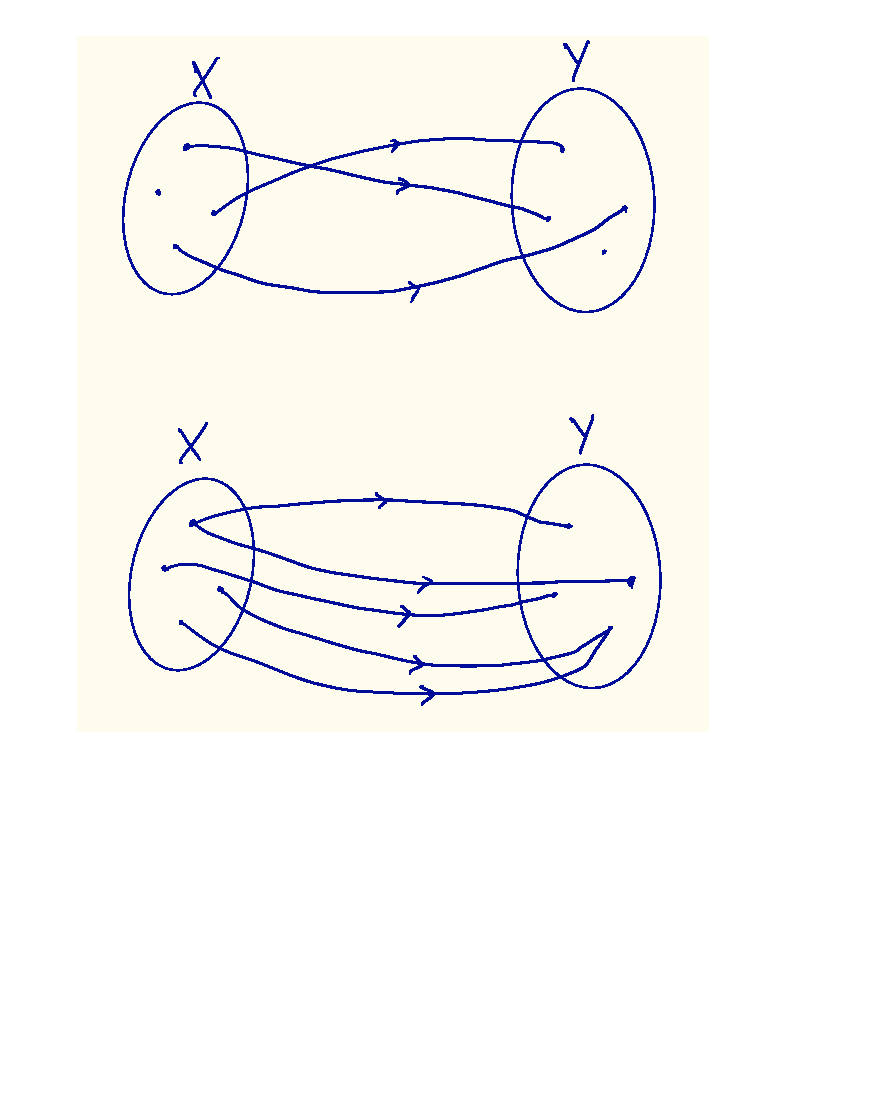
\includegraphics{images/non_functions}
            \caption{Two examples of non-functions. The first relation between $X$ and $Y$ is not a function, because not every element of $X$ is related to an element of $Y$. The second figure is not a function because there is an element of $X$ related to two elements of $Y$.}
            \label{fig:non_functions}
        \end{figure}

    \subsubsection{Classification of functions}
        By now, we have seen some examples of functions. In order to classify functions, we will introduce the terms surjection, injection, and bijection. For a visual overview of the terms, see Figure \ref{fig:sur_in_bi}. \\

        A function is called surjective (or: onto), if every element of its codomain is mapped to. \emph{Sur} means `above', which relates to the fact that the function's codomain is completely covered. Its definition can be written as follows: a function $f$ is said to be surjective if
        \begin{equation}
            f: X \rightarrow Y: \forall y \in Y: \exists x \in X: f(x) = y \thinspace .
        \end{equation}

        A function is called injective (or: one-to-one) if no element of its codomain is mapped to twice. Mathematically, we would write: $f$ is an injective function if
        \begin{equation}
            f: X \rightarrow Y: \forall a, b \in X: f(a) = f(b) \Rightarrow a = b \thinspace .
        \end{equation}

        A function is called bijective (or: one-to-one and onto, a one-to-one correspondence), if it is both injective and surjective: every element of the codomain is mapped to by exactly one element of the domain. \\

        The identity function on a set $S$ is the function:
        \begin{equation}
            \id_S: S \rightarrow S: \id_S(s) = s \thinspace .
        \end{equation}

        \begin{figure}[H] \centering
            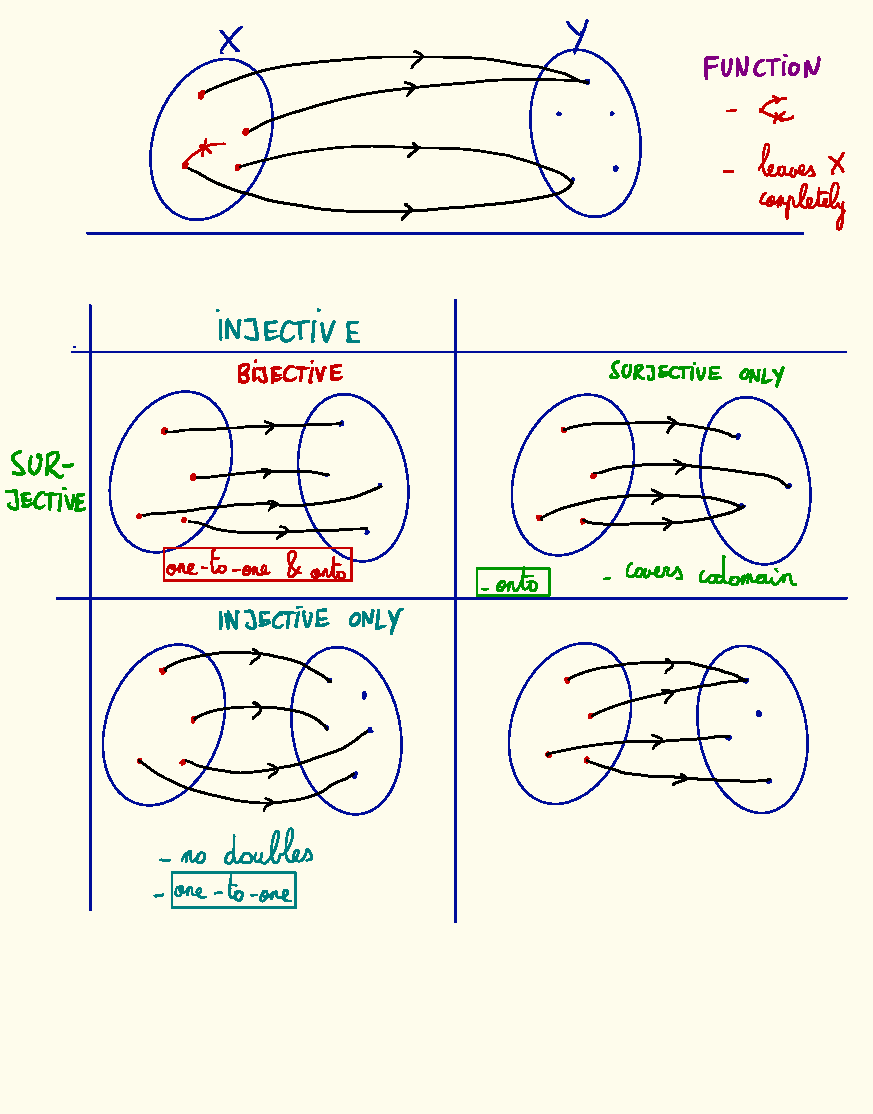
\includegraphics{images/sur_in_bi}
            \caption{A visual scheme of the terms surjective, injective and bijective.}
            \label{fig:sur_in_bi}
        \end{figure}

        Given Figure \ref{fig:sur_in_bi}, we can already see examples of surjective and injective functions. In Figure \ref{fig:function_color}, we can see an example of a function that is not surjective (not every color is mapped to), nor injective (the color red is mapped to twice). \\

    \subsubsection{More types of functions}
        An operation is a special kind of function. It is a function
        \begin{equation}
            \omega: X^n \rightarrow X \thinspace ,
        \end{equation}
        which takes $n$ elements from the set $X$ as input, and relates that combination to the set $X$ itself. \\

        We know many operations, for example number addition, which takes two numbers as input and relates that combination to another number. Number multiplication is another example of a binary operation: we take two numbers, whose product is another number. The set $X$ is not confined to be a set of numbers. If we take, for example, set of $n \times n$ matrices, then matrix multiplication is an example of a binary operation. \\
